\documentclass[12pt,a4paper]{article}
% Estilo compartido para informes. Compilar con LuaLaTeX desde tp1/.
\usepackage[spanish,es-nodecimaldot]{babel}
\usepackage{fontspec}
\setmainfont{Montserrat-Medium.ttf}[
  Path=../assets/fonts/,
  BoldFont=Montserrat-Bold.ttf,
  ItalicFont=Montserrat-MediumItalic.ttf]
\usepackage[a4paper,margin=2.5cm,headheight=16pt]{geometry}
\usepackage{xcolor,graphicx,booktabs,tabularx}
\usepackage{float}
\usepackage{titlesec,fancyhdr,enumitem,caption}
\usepackage{ragged2e}
\usepackage{hyperref}
\definecolor{verde}{HTML}{1D4036}
\definecolor{bronce}{HTML}{D38129}
\definecolor{rosa}{HTML}{D88E77}
\definecolor{calido}{HTML}{EFE4D8}
\definecolor{grafito}{HTML}{1D1D1D}
\hypersetup{colorlinks=true,linkcolor=verde,urlcolor=verde,
  pdftitle={TP1 - Instalación de máquinas virtuales},pdfsubject={Cyberseguridad}}
\AtBeginDocument{\color{grafito}\RaggedRight\fontsize{12}{14.4}\selectfont}
\setlength{\parindent}{0pt}
\setlength{\parskip}{7pt}
\setlist[itemize]{leftmargin=*,itemsep=7pt,topsep=4pt}
\setlist[enumerate]{leftmargin=*,itemsep=6pt}
\titleformat{\section}{\color{verde}\bfseries\fontsize{18}{21.6}\selectfont}{\thesection}{0.65em}{}
\titleformat{\subsection}{\color{verde}\bfseries\large}{\thesubsection}{0.65em}{}
\titleformat{\subsubsection}{\color{verde}\bfseries}{\thesubsubsection}{0.65em}{}
\titlespacing*{\section}{0pt}{16pt}{8pt}
\titlespacing*{\subsection}{0pt}{12pt}{5pt}
\titlespacing*{\subsubsection}{0pt}{10pt}{4pt}
\setcounter{tocdepth}{2}
\pagestyle{fancy}
\fancyhf{}
\fancyhead[L]{\small\color{verde}FCEFyN | UNC}
\fancyhead[R]{\small\color{verde}\materia\ · TP \numeroTP}
\fancyfoot[L]{\scriptsize Informe de laboratorio}
\fancyfoot[R]{\small\thepage}
\renewcommand{\headrulewidth}{0.4pt}
\captionsetup{font=small,labelfont=bf,justification=raggedright,singlelinecheck=false,hypcap=false}
\newcommand{\pendiente}[1]{\par{\small\color{verde}\textbf{Por completar.} #1\par}}
% Si falta una captura se muestra un espacio reservado; no impide compilar.
\newcommand{\captura}[2]{%
  \par\smallskip\begingroup\centering
  \IfFileExists{figuras/#1}{%
    \includegraphics[width=\linewidth,height=5cm,keepaspectratio]{figuras/#1}%
  }{%
    \setlength{\fboxsep}{10pt}%
    \fcolorbox{bronce}{calido}{\parbox[c][1.25cm][c]{\dimexpr\linewidth-2\fboxsep-2\fboxrule\relax}{%
      \centering\small Captura pendiente\par\texttt{\detokenize{#1}}}}%
  }%
  \captionof{figure}{#2}\par\endgroup\smallskip
}

\usepackage{xurl}

\newcommand{\materia}{Cyberseguridad}
\newcommand{\numeroTP}{4}
\newcommand{\tituloTP}{NTP, NTPsec y NTS}
\newcommand{\estudiante}{Brigido Tomas Andres}
\newcommand{\legajo}{38481096}
\newcommand{\carrera}{ICOMP}
\newcommand{\docente}{Javier A. Jorge}


% Metadatos específicos del TP4 y capturas en img/.
\hypersetup{pdftitle={TP4 - NTP, NTPsec y NTS}}
\renewcommand{\captura}[2]{%
  \begin{figure}[H]
    \centering
    \IfFileExists{img/#1}{%
      \includegraphics[width=0.85\linewidth,height=5cm,keepaspectratio]{img/#1}%
    }{%
      \setlength{\fboxsep}{10pt}%
      \fcolorbox{bronce}{calido}{\parbox[c][1.1cm][c]{0.85\linewidth}{%
        \centering\small Captura pendiente\par\texttt{\detokenize{#1}}}}%
    }%
    \caption{#2}
  \end{figure}
}

\begin{document}
\hypersetup{pageanchor=false}
\begin{titlepage}
  
\includegraphics[width=8cm]{../assets/logo-fcefyn-2026.png}
  \vspace{1cm}

  {\color{verde}\small UNIVERSIDAD NACIONAL DE CÓRDOBA\par}
  \vspace{2.1cm}
  {\color{bronce}\bfseries\large TRABAJO PRÁCTICO \numeroTP\par}
  \vspace{0.45cm}
  {\color{verde}\bfseries\fontsize{32}{38.4}\selectfont NTP, NTPsec\\y NTS\par}
  \vspace{0.65cm}
  {\large \materia\par}
  \vspace{0.8cm}
  {\color{bronce}\rule{2.7cm}{2pt}\par}
  \vfill
  \renewcommand{\arraystretch}{1.45}
  \begin{tabular}{@{}p{3.2cm}p{10cm}@{}}
    Estudiante & \estudiante \\
    Legajo & \legajo \\
    Carrera & \carrera \\
    Docente & \docente \\
  \end{tabular}
  \vfill
  {\small Córdoba, Argentina\par}
\end{titlepage}
\hypersetup{pageanchor=true}

\tableofcontents
\vspace{1cm}
\newpage

\section{Introducción y objetivos}
Este trabajo estudia la seguridad de la sincronización horaria mediante NTP.
La consigna propone analizar vulnerabilidades y sus consecuencias, revisar
la configuración del equipo y evaluar defensas con NTPsec y NTS en un
escenario de laboratorio aislado.
\begin{itemize}
    \item Investigar las vulnerabilidades de NTP y sus posibles impactos.
    \item Documentar la configuración horaria actual y su verificación.
\end{itemize}

\section{Preguntas y actividades}
\begingroup
\renewcommand{\arraystretch}{1.4}
\begin{tabularx}{\linewidth}{@{}p{2.5cm}>{\RaggedRight\arraybackslash}X@{}}
\toprule
\textbf{Término} & \textbf{Qué es} \\
\midrule
\textbf{NTP} & El protocolo que permite sincronizar relojes por la red. \\
\textbf{NTPsec} & Una implementación de NTP enfocada en seguridad. \\
\textbf{NTS} & Un mecanismo que agrega autenticación criptográfica a la sincronización mediante NTP. \\
\bottomrule
\end{tabularx}
\endgroup

\begin{enumerate}
    \item \textbf{¿Cuáles son las vulnerabilidades de NTP? ¿Qué implicancias podría tener su explotación?}

    Algunas de las principales bulnerabilidades de NTP incluyen ataques de amplificación DDoS,
    ciertos comandos de gestion NTP permiten a un atacante hacer que el servidor NTP responda con una
    cantidad mucho mayor a la vitctima y saturar su ancho de banda.
    
    Otra vulnerabilidad importante es la falsificacion de direccion IP, esto permite a un atacante
    enviar paquetes NTP falsos simulando ser un servidor NTP confiable.

    \newpage
    \item \textbf{¿Cuál es la configuración actual de NTP en tu equipo?}
    \begin{figure}[H]
      \centering
      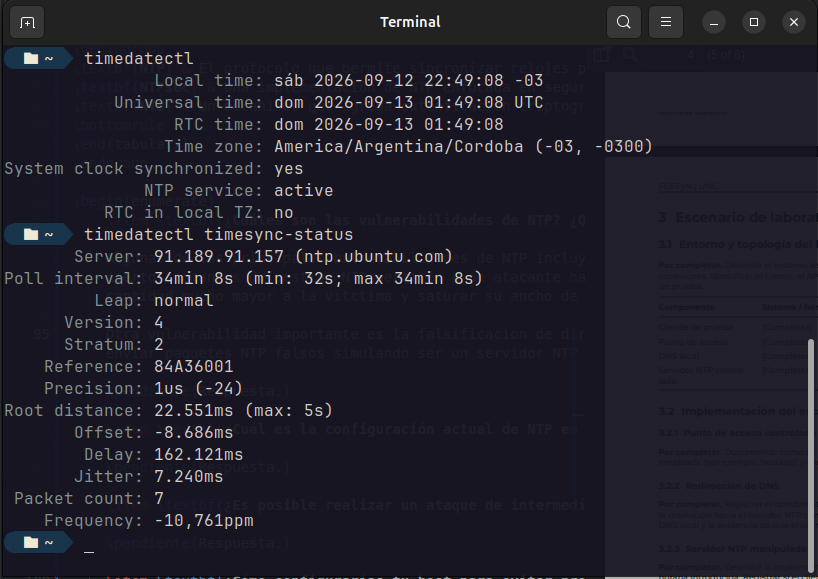
\includegraphics[width=0.85\textwidth]{img/timeprotocol.png}
      \caption{Configuración de NTP.}
      \label{fig:imagen}
    \end{figure}

    \item \textbf{¿Es posible realizar un ataque de intermediario (MITM) sobre un servicio NTP? ¿Podés implementarlo en el entorno aislado del laboratorio?}

   Sí, es totalmente posible realizar un ataque de intermediario (MITM) sobre el protocolo NTP, principalmente porque las versiones más utilizadas de NTP (como NTPv4) no implementan cifrado ni autenticación de forma predeterminada. Esto permite a un atacante interceptar y modificar los paquetes de tiempo para alterar el reloj de la víctima.

    \item \textbf{¿Cómo configurarías tu host para evitar problemas con NTP? ¿Cómo verificarías que la configuración es correcta?}
    
    Mantendría actualizado el cliente NTP y usaría servidores compatibles con NTS para autenticar las respuestas. Verificaría en el estado y los registros del servicio que el reloj esté sincronizado, que se utilice el servidor configurado y que la autenticación NTS esté activa.

    \item \textbf{¿Conocés ntp.inti.gob.ar? ¿Es seguro?}
    Es el servidor de INTI que proporciona servicios de sincronización horaria basada en operacion de un conjunto de relojes atomicos. Su seguridad depende de la implementación y configuración del servidor, así como de la red en la que se encuentre. Para mayor seguridad, se recomienda utilizar servidores NTP que soporten NTS y estén actualizados.
\end{enumerate}

\section{Referencias}
\begin{enumerate}
    \item Consigna del TP4: \textit{NTP, NTPsec y NTS}, archivo
    \texttt{consigna.pdf} suministrado para la actividad.
    \item FCEFyN, Universidad Nacional de Córdoba. \textit{Manual de
    identidad visual}, 2026. Base del estilo del informe.
\end{enumerate}
\end{document}
